\documentclass[10pt,a4paper]{article}
\usepackage[english]{babel}
\usepackage[utf8]{inputenc}
\usepackage[T1]{fontenc}
\usepackage{listings}
\usepackage{gensymb}
\usepackage[ddmmyy]{datetime}
\usepackage{graphicx}
\usepackage{xcolor}
\usepackage{fancyvrb}
\usepackage{enumitem}
\usepackage{multirow}

%
% COMPILE USING PDFLATEX
%

\newcommand{\mnfysrppic}{\texttt{mn-fysrp-pic}}
\newcommand{\reffig}[1]{Fig.~\ref{fig:#1}}
\newcommand{\refapp}[1]{App.~\ref{app:#1}}
\newcommand{\refsec}[1]{Sec.~\ref{sec:#1}}
\newcommand{\reftab}[1]{Tab.~\ref{tab:#1}}
\renewcommand{\dateseparator}{.}
%\def\labelitemi{\tiny$\bullet$}
%\def\labelitemii{\tiny$\bullet$}
%\def\labelitemiii{\tiny$\bullet$}

\author{Sigvald~Marholm}
\title{Introduction to \mnfysrppic}
\date{\today}

\DefineVerbatimEnvironment{verbatim}{Verbatim}{xleftmargin=0in}

\lstdefinestyle{customc}{
  belowcaptionskip=1\baselineskip,
  breaklines=true,
  frame=l,
  xleftmargin=\parindent,
  language=C,
  showstringspaces=false,
  basicstyle=\footnotesize\ttfamily,
  keywordstyle=\bfseries\color{green!40!black},
  commentstyle=\itshape\color{purple!40!black},
  identifierstyle=\color{blue},
  stringstyle=\color{orange},
}

\lstset{language=C,style=customc,numbers=left}
%\lstset{language=bash}

\begin{document}

\maketitle
\newpage

\section{Introduction}
The \mnfysrppic{} Git repository holds the Particle-In-Cell (PIC) code PINC (Particle-IN-Cell) belonging to the 4Dspace project and the Plasma and Space Physics group at the Physics Department of UiO. In order to keep the code and its different versions clean and manageable and to avoid conflicts during cooperation it is of utmost importance that all users obey the rules of the repository. Each user is therefore responsible of making himself/herself familiar with the rules stated herein before contributing with any code, or before committing to the repository. Repeated failure to do so may result in reduced privileges or exclusion from the repository. To get access it is sufficient to read \refsec{access}, but it is expected that the developer is familiar with the rest before committing.



\section{Getting Access}\label{sec:access}
To access the repository and be able to make changes you need to set up a local copy. To get access you need an SSH key-pair (public and private keys). Unless you already have that you can run the following command\footnote{http://www.uio.no/tjenester/it/maskin/filer/versjonskontroll/git.html .}:

\begin{verbatim}
	ssh-keygen -t rsa -b 4096
\end{verbatim}
This generates the following files:

\begin{itemize}
	\item Private key: \verb$~/.ssh/id_rsa$
	\item Public key: \verb$~/.ssh/id_rsa.pub$
\end{itemize}
The private key is private (hence the name) and should under no circumstance be shared with others. It is what you use to authorize when logging into the remote server. The public key cannot be used to log in but is used by the remote server(s) to verify that you have the private key.

Rename a copy of your public key to \verb$<username>.pub$ where \verb$<username>$ is your UiO username, and mail it to the repository administrator (sigvaldm@fys.uio.no) and wait for approval.

Next, configure your local git user using these commands:

\begin{verbatim}
	git config --global user.name '<username>'
	git config --global user.email '<email>'
\end{verbatim}
Go to the folder where you'd like your local copy (typically your home directory), and clone the central repository (origin) like this:

\begin{verbatim}
	git clone gitolite@git.uio.no:mn-fysrp-pic
\end{verbatim}
A new folder with the name \verb$mn-fysrp-pic$ will be created. This is your local working copy.

If you want access from another computer (e.g.\ supercomputer) you have to copy your private key to \verb$~/.ssh/id_rsa$ on that computer, and run the configuration and cloning steps there as well. 

\section{Workflow}
The \mnfysrppic{} repository utilizes what's called a Feature Branch Workflow\footnote{See more about various Git workflows here: https://www.atlassian.com/git/tutorials/comparing-workflows .} as illustrated in \reffig{featurebranch}. The reason for this is to allow several users to develop functions for the code independently with a minimum of conflicts. It also assures that a fully functioning version of the code is always accessible. Using Git also means that all previous revisions of the code are retrievable. This, along with information on which revision was used to generate a set of results, make the experiments reproducible. 

To briefly explain the Feature Branch Workflow, the master branch should always represent a fully functional version of the PIC code. Whenever a new feature is to be developed a new feature branch (e.g. Feature 1 in the figure) is created and the user works on that branch until the feature is finished. Then, it is merged back onto the master branch. The user verifies that the master branch executes and is fully functioning before pushing the changes to the central repository (the origin). Ruining the central master branch causes trouble for other users who expect it to be up and running. 

Let's consider an example: One user starts implementing a new input settings system for the PIC code (Feature 2). At the same time another user starts revising the field solver (Feature 3). Each user can make as many commits as desirable within their feature branch for the sake of backup. The input system is finished first and its feature branch is merged back onto the master branch before being deleted. It doesn't matter that another user has edited parts of the field solver because that's in another branch. The master branch is now a fully functional PIC code with new input system but with the old solver left intact. Once the new solver is finished, it is merged back to the master. But the master has changed since the revision Feature 3 is built upon. These changes, however, most likely affect other files and Git will be able to seamlessly merge only the appropriate lines changed during Feature 3 development. If uncertainties occur, Git will ask the Feature 3 developer to do some manual work to properly merge Feature 3 with the master branch. Feature 2 will not be overwritten.

\begin{figure}
	\centering
	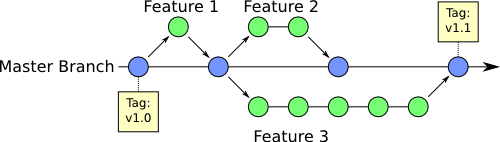
\includegraphics[width=0.8\textwidth]{featurebranch.png}
	\caption{Illustration of Feature Branch Workflow}
	\label{fig:featurebranch}
\end{figure}

Feature branches normally only exist locally. If desirable, they can be pushed to the central repository (the origin) to make them accessible from several computers (for instance for collaboration). The origin should be kept clean, however, meaning that someone must be responsible to delete the branches after merging ensuring that only a few branches exist centrally. Only the repository administrator has the privilege to delete branches and cleaning the origin so other users should ask for permission before pushing new branches to the origin. Moreover, the branches pushed to origin should have globally understandable names.

As a summary: feature branches can have many revisions allowing the developer to go back in case of mistakes, for backup, and for sharing code with other developers. The master branch is holy and only fully functional features should be merged into it.

If this section is unclear and more advice on Git is needed please refer to \texttt{mn-fysrp-pic/docs/git.pdf} before making any changes to the repository.

\section{Reproducibility}
It is currently a long term plan to release PINC as an open source project. Some revisions of PINC can then be tagged in Git with a version number, and authors of scientific publications can specify which version was used, thereby making the results truly reproducible by others, as is the spirit of science. Version tags should only be put on revisions on the master branch.

Moreover, it is a not-yet-implemented feature of PINC that an auxiliary file is output which states which version and revision of PINC was used to generate the results, which versions was used of third party libraries, and which hardware was used. This feature is supposed to fetch the version tag and the revision number automatically from Git.

\section{Repository Structure}

\subsection{Folder Structure}
The \mnfysrppic{} repository has the following folder structure (unimportant details omitted):

\begin{itemize}[label={}]
	\item \verb$mn-fysrp-pic/$
	\begin{itemize}[label={}]
		\item \verb$doc/$
		\begin{itemize}[label={}]
			\item \verb$doxygen/$
			\item \verb$html/$ (gitignored)
			\item \verb$introduction/$
			\item \verb$latex/$ (gitignored)
			\item \verb$introduction.pdf$ (this file)
		\end{itemize}
		\item \verb$lib/$
		\item \verb$proof of concept/$
		\item \verb$script/$
		\item \verb$src/$
%		\begin{itemize}[label={}]
%			\item \verb$main.c$
%			\item \verb$pinc.h$
%		\end{itemize}
%		\item \verb$check.sh$
		\item \verb$test/$
		\item \verb$input.ini$
		\item \verb$makefile$
		\item \verb$mpinc.sh$
		\item \verb$pinc$ (gitignored)
	\end{itemize}
\end{itemize}

\verb$doc$ contains documentation of the code and the repository. That includes this document (\verb$introduction.pdf$) along with a similarly named folder containing the \LaTeX{} source files used to create it. \verb$html$ and \verb$latex$ contains documentation of the code in HTML and LaTeX, respectively. This documentation is not, strictly speaking, part of the repository, but rather is auto-generated by Doxygen from the files in the repository when building the code. The \verb$doxygen$-folder includes auxiliary files needed by Doxygen to do this.

Small non-standard third party libraries are shipped with the code for convenience. They are put under the folder \verb$lib$ uncompressed but otherwise as provided by the manufacturer, i.e.\ uncompiled and with legal information files/licenses. Unfortunately, it has too many drawbacks to include big standard libraries in this folder and perform static linking even though this would've guaranteed consistent executions across computers. See \refsec{dependencies}.

The source code is located at \verb$src$ and it is the primary task of the repository is to act as a Version Control System (VCS) for the code (.c-files and .h-files) within this folder. The repository should not track object (.o) files, compiled and linked executables, binaries or similar (also true for third party libraries). VCSs like Git only needs to keep track of the lines changed in text files which makes them very efficient. Other files such as executables and object files carry no real information to the programmer and must be re-stored in entirety every time it changes (after each compilation). Many such files can make the repository heavy. It also clutters the repository with unnecessary changes each time someone recompiles the whole program, causing unnecessary Git conflicts. For this reason these file types are added to \verb$.gitignore$ which means that they will not be committed to the repository.

The folder \verb$proof of concept$ may be used to test smaller pieces of code, for instance to check the fastest way to implement something. If, for instance, it was found that one way of implementing something is faster than the other, it might be desirable to keep this experiment for future evidence. This folder is \emph{not} intended to store lots of old rubbish, it should exclusively be something that is clean enough to re-open and and (with little effort) refer to. \verb$old$ folders may \emph{temporarily} hold old files which are to be deleted once a replacement is developed.

\verb$test$ is the unit testing source files, to be more thoroughly documented at a later point, while \verb$script$ is a folder of Python scripts which are/can be used to visualize and interpret data. These are both useful for testing the code and for later starting points when doing simulations. Python scripts may also be used to do parameter sweeps by running PINC with several input parameters.

Finally, simulation .h5-files should not be part of the repository. They are incredibly large and there is also no reason to have version control on them; once a simulation is successfully run, and maybe even used in publications, it should be considered static. Simulations and their input files are also not, strictly speaking, part of the program.

\subsection{File Structure}
The PINC source files can be thought to belong to one of three categories as illustrated in \reftab{files}:

\begin{table}
	\centering
	\caption{Source file categorization}
	\begin{tabular}{|l l l|}
		\hline
										& .c-files 				& .h-files 							\\
		\hline \hline
		Main routine						& \verb$main.c$			&									\\
		\hline
		\multirow{4}{*}{Framework}		& \verb$aux.c$			& \multirow{4}{*}{\texttt{pinc.h}}	\\
										& \verb$grid.c$			&									\\
										& \verb$io.c$			&									\\
										& \verb$population.c$	&									\\
		\hline \hline
		Multigrid module					& \verb$multigrid.c$		& \verb$multigrid.h$					\\
		\hline
		\multirow{2}{*}{Future module}	& \verb$moduleA.c$		& \multirow{2}{*}{\texttt{module.h}}	\\
										& \verb$moduleB.c$		& 									\\
		\hline
	\end{tabular}
	\label{tab:files}
\end{table}

\verb$main.c$ is the main-routine, whereas \verb$pinc.h$ is the main header file declaring a framework for all PINC modules (pedantically it's not a framework but is thought of as such). It declares datatypes and functions for handling particles and grid quantities along with functions to manipulate them and other building block functions ensuring a coherent code. The definitions are stored in the accompanying .c-files. Modules, for instance a multigrid solver, act upon these standardized data structures, and is implemented in one .h-file and one or more .c-files starting with the name of the module. The framework files should \emph{not} depend on the modules.

%\section{Folder Structure (Deprecated)}
%For working with the PIC code, your home folder should have the following sub-folders (unimportant details omitted):
%
%\begin{itemize}
%	\item \verb$mn-fysrp-pic$
%	\begin{itemize}
%		\item \verb$DiP3D$
%		\begin{itemize}
%			\item \verb$template$
%			\item \verb$src$
%			\item \verb$lib$
%			\item \verb$doc$
%		\end{itemize}
%		\item \verb$docs$
%		\item \verb$proof of concept$
%	\end{itemize}
%	\item \verb$local_data$
%	\begin{itemize}
%		\item \verb$template$
%		\item \verb$YYMMDD_<simulation description 1>$
%		\item \verb$YYMMDD_<simulation description 2>$
%		\item \verb$...$
%	\end{itemize}
%\end{itemize}
%
%\verb$mn-fysrp-pic$ is the local working copy of the Git repository and is obtained by cloning the central repository as described in the previous section. \verb$mn-fysrp-pic/docs$ contain the documentation of the repository (including this document) along with files used to create the documentation.
%
%The source code for DiP3D is located at \verb$mn-fysrp-pic/DiP3D/src$. The primary task of the repository is to act as a Version Control System (VCS) for the code (.c-files) within this folder. The repository should not track object (.o) files, compiled and linked executables, binaries or similar. VCSs like Git only needs to keep track of the lines changed in text files which makes them very efficient. Other files such as executables and object files carry no real information to the programmer and must be re-stored in entirety every time it changes (after each compilation). Many such files can make the repository heavy. It also clutters the repository with unnecessary changes each time someone recompiles the whole program, causing unnecessary Git conflicts. For this reason these file types are added to \verb$.gitignore$.
%
%Third party, non-standard, libraries are shipped with the code in order to ensure consistent compilations amongst developers and on supercomputers. They are stored in \verb$mn-fysrp-pic/DiP3D/lib$ the way they are provided by the vendor, including necessary legal information.
%
%Compilation of DiP3D is performed by running the makefile in \verb$mn-fysrp-pic/DiP3D$. This also executes the makefiles of third party libraries, and auto-generates documentation of all C-functions in \verb$mn-fysr-pic/DiP3D/doc$ using Doxygen. Both HTML and LaTeX-documentation is generated. 
%
%The \verb$mn-fysrp-pic/proof of concept$ folder is used to test smaller parts that shall later be part of the program.
%
%\emph{Note: The folder structure is partly an inheritance from old DiP3D which looks for files with a hard-coded path two steps up. A new main routine is being developed and once that is finished the folder structure will be flattened and simplified. The program will also likely be named PINC (Particle-IN-Cell).}
%
%Simulation data files should also not be part of the repository. They are incredibly large and there is also no reason to have version control on them; once a simulation is successfully run, and maybe even used in publications, it should be considered static. Simulations and their input files are also not, strictly speaking, part of the program. For this reason the \lstinline$local_data$ folder can be created as follows:
%
%\begin{lstlisting}
%	cd mn-fysrp-pic
%	./setup_folders.sh
%\end{lstlisting}
%
%All the simulation-specific files are stored in sub-folders in \lstinline$local_data$ in order to separate it from the repository. Each simulation has exactly one sub-folder, which should be named \lstinline$YYMMDD_<simulation description>$ where YYMMDD is the date in reverse order. The sub-folders will contain the simulation results, as well as all the information necessary in order to make the numerical experiment reproducible: input files, job script, and information on exactly which Git revision of DiP3D was used to generate the result.
%
%After simulation is done, the simulation data sub-folders should be copied to \lstinline$some_server.uio.no/path/to/DiP3D_data/$ (TBD: folder not created yet). This server is automatically backuped by the IT department.
%
%The \lstinline$local_data/template$ folder contains example input files which serves as a starting point for making new simulation results. It is simply a copy of \lstinline$mn-fysrp-pic/DiP3D/template$. If for instance the format of the input files change, the template in the repository can be updated and \lstinline$setup_folders.sh$ can be run again to renew \lstinline$local_data/template$. All previously existing files in \lstinline$local_data/template$ will then be deleted, but all other files in \lstinline$local_data$ will persist.
%
%\emph{Note: The local\_data folder will soon be deprecated when the new main routine is finished.}
%
%\section{Running a Simulation (Deprecated)}
%\emph{Note: Ignore this section. It will be replaced once PINC is ready.}
%
%Running a DiP3D simulation while keeping folders clean is easily done as described in this section.
%
%First, you should checkout from Git the revision of DiP3D you'd like to use. Next, a new simulation data folder must be made. Here, we use the template as a starting point (a previously run simulation would also work):
%
%\begin{lstlisting}
%	cd local_data
%	cp -r template 150611_test_simulation
%	cd 150611_test_simulation
%\end{lstlisting}
%For the time being, the template contains the input files input.txt and sphere.txt which is edited according to the simulation in quest.
%
%\subsection{Abel Supercomputer}
%Next, to execute the job on Abel the job script \lstinline$start_abel$ is edited according to the users demands (with respect to resource usage and such) and executed:
%
%\begin{lstlisting}
%	sbatch start_abel
%\end{lstlisting}
%
%The job script copies all DiP3D source files and input files to Abel's scratch area before building the source and executing the simulation. This is the procedure recommended by USIT since the scratch area is faster. The simulation results are copied back to the data sub-folder after execution. This is true even if the program is terminated unexpectedly. The job scripts also generates a file called \lstinline$execinfo.txt$ which contains information about exactly which Git revision of DiP3D was used to produce the results, as fetched from Git itself. The file \lstinline$ompiinfo.txt$ contains the output of the bash command \lstinline$ompi_info$ showing information on versions of OpenMPI, compilers and miscellaneous. SLURM also writes its output file to this folder.
%
%Abel will automatically delete the scratch folder including all object files and executables. Neither the repository nor the \lstinline$local_data$ folder will be cluttered with these files. Finally, you should take a copy of the data sub-folder to \lstinline$some_server.uio.no/path/to/DiP3D_data/$ (TBD: folder not created yet)
%
%\subsection{Desktop Computer}
%On a plain desktop computer the code can be run without MPI like this:
%
%\begin{lstlisting}
%	./start_plain.sh
%\end{lstlisting}
%
%\lstinline$start_plain.sh$ creates a scratch folder within the data folder which acts the same way as scratch on Abel. This folder is deleted if the execution script is successfully run. The information files are generated also in this case.

\section{Compiling and Running PINC}\label{sec:dependencies}
Before being able to compile PINC the following libraries must be installed:
\begin{enumerate}
	\item OpenMPI
	\item GNU Scientific Library (GSL)
	\item HDF5 API including parallel support (more on parallel support later)
\end{enumerate}
These are typically installed either through \verb$sudo apt-get install$ when available or by downloading the source code and executing something like this:

\begin{verbatim}
	./configure
	make
	sudo make install
\end{verbatim}
The last step is crucial since this makes the system find the library without having to add local modifications to the PINC makefile. While it is permitted to do whatever you like locally, it is not permitted to push files of local relevance only to origin, and it is therefore advised to install the libraries on the system.

Once dependencies are resolved PINC is compiled using the makefile in the repository:

\begin{verbatim}
	cd mn-fysrp-pic
	make
\end{verbatim}
The makefile installs the libraries in \verb$lib$ as well as generating Doxygen documentation. When adding new header or source files these can be added to \verb$HEAD_$ or \verb$SRC_$, respectively, in the makefile. Next, PINC is executed as

\begin{verbatim}
	./pinc input.ini
\end{verbatim}
where \verb$input.ini$ tells PINC which settings to use. More than one process can be run in the normal way using \verb$mpirun$ as illustrated below (for two processes):

\begin{verbatim}
	mpirun -np 2 pinc input.ini
\end{verbatim}
however, the number of subdomains to use in the domain decomposition must correspond to the number of processes. If, for instance, you have $4\times 4\times 4$ subdomains specified in \verb$input.ini$, the number of processes must be 64. This command can be run more simply as:

\begin{verbatim}
	./mpinc.sh input.ini
\end{verbatim}
which extracts the number of processes required by PINC and automatically sets the \verb$np$ parameter of \verb$mpirun$.

PINC is more kind of a numerical ``engine'' than a tool for diagnostics, parameter sweeps and so on. To facilitate parameter sweeps performed by external (Python) scripts, parameters in the input file can be overridden through additional command line arguments to PINC, following the following syntax:
\begin{verbatim}
	./mpinc.sh input.ini <section>:<key>=<value> <section>:<key>=<value> ...
\end{verbatim}
For instance, the number of subdomains to use is specified as the parameter \verb$nSubdomains$ under the section \verb$grid$ in \verb$input.ini$. To override the input file and specify $4\times 4\times 4$ subdomains, call the following command:

\begin{verbatim}
	./mpinc.sh input.ini grid:nSubdomains=4,4,4
\end{verbatim}
Unfortunately, a value for \verb$nSubdomains$ must already be set in \verb$input.ini$ to be able to override it through the command line (this is due to a limitation of the third party library).

Finally, to erase all build files run
\begin{verbatim}
	make clean
\end{verbatim}

\section{Tools}
This section describes tools that can be useful for developers.

\subsection{Editor}
Use whichever editor you want (I use Atom) but do not clutter the repository with editor files. Also, make sure the editor settings obey the coding conventions with respect to spaces, tab sizes, etc.

\subsection{Doxygen}
As already mentioned, the code is documented using Doxygen. Build PINC and the documentation will be at \verb$mn-fysrp-pinc/doc/html/index.html$.

\subsection{Unit Testing}
To run unit tests, execute the following command:

\begin{verbatim}
	make test
\end{verbatim}
which will build a unit test executable \verb$ut$ and execute it. How to develop unit tests is briefly described in Doxygen.

\subsection{Valgrind}
To ensure that dynamically allocated memory is freed use Valgrind. Since OpenMPI generates a lot of false positives these false positives are suppressed by using the PINC wrapper script \verb$valgrind.sh$ for running Valgrind instead of just \verb$valgrind$\footnote{Since OpenMPI is usually not compiled with \texttt{--enable-memchecker} Valgrind will not be able to detect errors in shared memory space. I guess most (all?) mistakes will be eliminated using the PINC Valgrind wrapper, however.}. First, make sure Valgrind is installed on your system. Then, consider the following example:

\begin{lstlisting}
void test(){
	char *ptr = malloc(1048576);
}

int main(int argc, char *argv[]){

	char *str = malloc(16);
	strcpy(str,"test");
	
	test();

	printf("%s\n",str);
	return 0;
}
\end{lstlisting}
Then, compiling and running valgrind as follows:

\begin{verbatim}
	make clean
	make COPT=
	./valgrind.sh ./pinc input.ini
\end{verbatim}
returns (uninteresting details removed):

\begin{verbatim}
HEAP SUMMARY:
    in use at exit: 1,255,872 bytes in 498 blocks
  total heap usage: 7,251 allocs, 6,753 frees, 14,389,316 bytes allocated

16 bytes in 1 blocks are definitely lost in loss record 88 of 340
   at 0x4C2AB80: malloc (in /usr/lib/valgrind/vgpreload_memcheck-amd64-linux.so)
   by 0x40166D: main (in /home/sigvald/mn-fysrp-pic/pinc)

1,048,576 bytes in 1 blocks are definitely lost in loss record 340 of 340
   at 0x4C2AB80: malloc (in /usr/lib/valgrind/vgpreload_memcheck-amd64-linux.so)
   by 0x40164E: test (in /home/sigvald/mn-fysrp-pic/pinc)
   by 0x401685: main (in /home/sigvald/mn-fysrp-pic/pinc)

LEAK SUMMARY:
   definitely lost: 1,048,592 bytes in 2 blocks
   indirectly lost: 0 bytes in 0 blocks
   possibly lost: 0 bytes in 0 blocks
   still reachable: 0 bytes in 0 blocks
   suppressed: 207,280 bytes in 496 blocks

For counts of detected and suppressed errors, rerun with: -v
ERROR SUMMARY: 2 errors from 2 contexts (suppressed: 53 from 53)
\end{verbatim}

This shows that \lstinline$malloc()$ in \lstinline$main()$ allocated 16 bytes which is not freed, and that \lstinline$malloc()$ in \lstinline$test()$ in \lstinline$main()$ allocated 1MiB which is not freed. It also showed that approximately 200KiB which is not freed is suppressed. This is not due to PINC mistake but due to OpenMPI and is therefore not considered an error. Except for the suppressed leaks all leaks should be zero. Feel free to read more about the different leaks online.

The \verb$COPT=$ argument in the make-call above is used to turn off compiler optimizations. Without this, the compiler would figure out that the function \lstinline$test()$ does nothing and can be omitted. As a result, only the first error would show up. In fact, the second error does not exist any more after optimizing and therefore pose no problems. Nevertheless, it may be helpful to turn off optimizations when looking for memory leaks.

Finally, beware that running Valgrind degrades execution speed.

%To be able to run Valgrind memchecker for parallel applications without false positive errors OpenMPI needs to be installed with support for memchecker enabled. This makes OpenMPI perform slightly slower, but is useful for using Valgrind to test for memory leaks.
%
%Make sure valgrind is installed using \verb$sudo apt-get install valgrind$. If the \verb$valgrind$ command works it is installed. Next, download OpenMPI source code and compile a memchecker-enabled version of it like this:
%
%\begin{verbatim}
%	./configure --prefix=/path/to/install/openmpi --enable-debug \
%	--enable-memchecker --with-valgrind=/path/to/valgrind
%	make
%	sudo make install
%\end{verbatim}
%On Ubuntu, \verb$/path/to/valgrind$ is typically \verb$/usr$, since make will then look for include-files in \verb$/usr/include/valgrind/$ and so on. \verb$sudo make install$ may be executed to install it globally, but if you'd like to keep the higher-performance non-valgrind OpenMPI available you may skip this.
%
%Warning: On computers with OpenMPI already installed, it is possible that this newly compiled OpenMPI is not the one that is used when executing \verb$mpirun$ and such. To remedy this go to the folder where it is installed. Execute the following command:
%\begin{verbatim}
%	./ompi_info 	| grep memchecker
%\end{verbatim}
%
%If OpenMPI was successfully built for using valgrind it should look something like this:
%\begin{verbatim}
%	 MCA memchecker: valgrind (MCA v1.0, API v1.0, Component v1.3)
%\end{verbatim}

\subsection{GProf}
To get an overview of what is time-consuming in PINC, execute the following commands:

\begin{verbatim}
	make clean
	make CADD=-pg
	./pinc input.ini
\end{verbatim}
\verb$CADD$ is used to add additional flags to the compiler. In this case instrumentation code is incorporated into PINC to allow GProf to profile it. Upon execution of PINC the file \verb$gmon.out$ (gitignored) is created which can be analysed with GProf. Extensive documentation of GProf is available online but as an example,

\begin{verbatim}
	gprof -bap pinc gmon.out
\end{verbatim}
may return

\begin{verbatim}
Flat profile:

Each sample counts as 0.01 seconds.
  %   cumulative   self              self     total           
 time   seconds   seconds    calls  ms/call  ms/call  name    
100.04      0.96     0.96        3   320.14   320.14  posUniform
  0.00      0.96     0.00       36     0.00     0.00  intArrMul
  0.00      0.96     0.00       22     0.00     0.00  iniGetStrArr
  0.00      0.96     0.00       14     0.00     0.00  intArrProd
  0.00      0.96     0.00        7     0.00     0.00  iniGetLongIntArr
  0.00      0.96     0.00        6     0.00     0.00  msg
  0.00      0.96     0.00        3     0.00     0.00  iniGetIntArr
  0.00      0.96     0.00        2     0.00     0.00  iniGetDoubleArr
  0.00      0.96     0.00        1     0.00     0.00  allocGrid
  0.00      0.96     0.00        1     0.00     0.00  allocPopulation
  0.00      0.96     0.00        1     0.00     0.00  tFormat
  0.00      0.96     0.00        1     0.00     0.00  velMaxwell
\end{verbatim}

Mind that a significant amount of time is necessary in order for GProf to be able to determine non-zero time.

\subsection{Simple Timing using PINC \texttt{Timer}}
While GProf is suitable to get an idea of the execution of the whole program it has its flaws. One of them is when you want to know rigorously how fast certain operations execute. For this purpose, the PINC \texttt{Timer} datatype may come in handy. Consider for instance that you know two different ways of implementing the same thing, one intuitive way using nested loops, and one ``clever'' way using one loop and a modulo operator. These can be compared as shown below:

\begin{lstlisting}
	Timer *timer = allocTimer(0);

	int nDims = 3;
	int L[3] = {1,2,4};
	double *pos = pop->pos;

	tMsg(timer,NULL);
	
	for(long int i=0; i<1e7; i++){
		for(int d=0;d<nDims;d++){
			pos[i*nDims+d] = L[d]*gsl_rng_uniform_pos(rng);
		}
	}
	
	tMsg(timer,"Nested loops method");

	for(long int i=0; i<nDims*1e7; i++){
		pos[i] = L[i%nDims] * gsl_rng_uniform_pos(rng);
	}
	
	tMsg(timer,"Modulus method");

	freeTimer(timer);
\end{lstlisting}

Then compiling with
\begin{verbatim}
	make clean
	make
	./pinc input.ini
\end{verbatim}
returns

\begin{verbatim}
TIMER (0): [tot=332.81ms, diff=289.26ms] Nested loops method
TIMER (0): [tot=619.69ms, diff=286.83ms] Modulus method
\end{verbatim}
\verb$tot$ shows the time since program start-up whereas \verb$diff$ shows time since previous invocation of \lstinline$tMsg()$. \lstinline$tMsg(timer,NULL)$ can be called simply to reset the timer without printing any message.

In this case, we see that both methods perform equally well at approximately 290~ms. The difference is insignificant. It is interesting though, to re-run the experiments with optimizations turned off (``\verb$make COPT=$''):

\begin{verbatim}
TIMER (0): [tot=397.32ms, diff=359.46ms] Nested loops method
TIMER (0): [tot=956.03ms, diff=558.67ms] Modulus method
\end{verbatim}
It is now evident that the intuitive nested loops method by itself is faster but the compiler has optimized both methods such that they perform similarly. This information, however, is purely for educational purpose, as it is no point in optimizing the code with compiler optimizations turned off. The rationale is; if two alternatives perform equally well with compiler optimizations on, choose the prettiest solution. If not, choose the fastest.

Whereas this example was well optimized by the compiler, this may not always be the case. It is therefore highly advised to think through your programming techniques, and when uncertain as to what will perform well, measure it.

As a final note, although the PINC Timer has a very high resolution the accuracy is more influenced by random variations and overhead when measuring short times. A remedy to this is to put the operations to be measured in a loop to get the timer up to the the millisecond range. To get an idea of the resolution, the overhead and the accuracy of \lstinline$tMsg()$ try measuring \lstinline$tMsg()$ itself by running it in a loop\footnote{Technically the timer is measured at the beginning of \lstinline$tMsg()$ and reset at the end of \lstinline$tMsg()$ such that \texttt{diff} actually shows the time between, but not including, calls to \lstinline$tMsg()$. This gives more accurate readings of what comes in between. On my computer \lstinline$tMsg()$ executes in approximately $5 \mu s$ but the overhead of the measurements is only approximately 200~ns. The discrepancy is largely due the fact that printing to the terminal takes time.}.

\subsection{GNU Debugger (GDB)}
GDB may be useful if for instance you want to step through your code, inspecting what's happening to variables as the program run. To be able to use GDB the program must be compiled with the additional \verb$-g$ flag as follows:

\begin{verbatim}
	make clean
	make CADD=-g
	gdb pinc
\end{verbatim}
from which point you can use GDB. GDB is well documented online. Beware that sometimes things may look strange due to optimizations, for instance the value of a variable may not exist and show up as ``<optimized out>'', either because it simply is not needed, or because it is not needed at this point. As usual, you can turn off optimization for debugging purposes by running \verb$make CADD=-g COPT=$.

\section{Coding Practices}
Herein is described the coding conventions to be used within the project.

\subsection{Naming Conventions}
We use the camelCase-convention rather than underscore. E.g:
\begin{lstlisting}
int myVariable = 0;
void myFunction();
\end{lstlisting}
Names should be intuitive rather than short. On the other hand, too long names are bothersome too. Obvious abbreviations are okay. Common abbreviations and names are okay too even if hard to read simply because their commonness makes them more likely to be understood than easier but unfamiliar names. Examples:
	\begin{itemize}
		\item \lstinline$knErg$ is a worse name than \lstinline$kineticEnergy$ which is a worse name than \lstinline$energy$ (if kinetic energy is the only kind of energy that makes sense).
		\item \lstinline$wij1k1$ is a horrible name.
		\item \lstinline$temp$ is a perfectly understandable name for a temporary variable inside a sufficiently short scope. No need to call it \lstinline$kineticEnergyFromPreviousTimeStep$. \lstinline$temp2$ however is usually a sign that you need to clean up.
		\item \lstinline$i$ and \lstinline$j$ are perfect names for a loop counters. No need to call it \lstinline$loopCounter$. Make sure to avoid confusion with common uses of \lstinline$i$ and \lstinline$j$ in PINC, though.
		\item \lstinline$argc$ and \lstinline$argv$ are okay since they are understood by any C programmer.
		\item \lstinline$pos$ is okay since it's obviously a contraction of ``position''.
	\end{itemize}
Generally speaking, the larger the scope a variable or function has the more important is its proper naming.
\subsubsection{Grammar}
Moreover we have the following grammar conventions:
		\begin{itemize}
			\item \lstinline$nElements$. ``n'' in the beginning of a variable name like this is read like ``the number of''. The word(s) that come after ``n'' should be plural. You don't say ``the number of element''.
			\item In many cases it is a good idea that arrays have plural names. Consider this example:
\begin{lstlisting}
int numbers[100];
for(int i=0;i<100;i++){
	int number = numbers[i];
	// Do something with "number"
}
\end{lstlisting}
			\item Because of the above point, datatypes (and structs) should have singular names. Consider these examples
\begin{lstlisting}
// CORRECT (if the struct contains only one particle)
Particle particles[100];

// WRONG: This is just confusing.
Particles particless[100];

// CORRECT. Each element is a population of particles.
Population pops[100];
\end{lstlisting}
		\end{itemize}

\subsubsection{Structs}
Structs are named with a capital first letter to indicate that it is a struct:

\begin{lstlisting}
typedef struct{
	...
} MyStruct;
\end{lstlisting}
More precisely, we actually do \emph{not} give the struct a name, but rather name its datatype using \lstinline$typedef$. Naming the struct would look something like this:

\begin{lstlisting}
// WRONG
typedef struct MyStruct{
	...
} MyStruct;
\end{lstlisting}
or:
\begin{lstlisting}
// WRONG
struct MyStruct{
	...
};
typedef struct MyStruct MyStruct;
\end{lstlisting}
Naming \emph{both} the struct and the datatype means that the same variable could be declared using two notations and we strive for consistency:

\begin{lstlisting}
MyStruct newInstance;		// CORRECT
struct MyStruct newInstance;	// WRONG
\end{lstlisting}
The only exception I can think of when naming the struct itself is necessary is when using opaque datatypes, if that will ever be relevant.

\subsubsection{Indices}
In numerical codes there are often many indices. As an effort to avoid confusion one should not use one variable name for loop counter of particles one place and for grid another place. \reftab{suggested_names} shows names which are to be used for loops through grids or particles along with comparisons to how they could be written mathematically.

\begin{table}
	\centering
	\caption{Suggested names in PINC}
	\begin{tabular}{|l|c|c|}
		\hline
										& C 							& Math			\\
		\hline \hline
		time step						& \lstinline$n$				& $n$			\\
		number of time steps				& \lstinline$nTimeSteps$		& $N_t$			\\
		\hline
		dimension						& \lstinline$d$				& $d$			\\
		number of dimensions				& \lstinline$nDims$			& $N_d$			\\
		\hline
		specie							& \lstinline$s$				& $s$			\\
		number of species				& \lstinline$nSpecies$		& $N_s$			\\
		\hline
		particle index					& \lstinline$i$				& $i$			\\
		number of particles				& 							& $N_p$			\\
		\hline
		node index within local MPI subdomain	& \lstinline$p=func(j,k,l)$			& $p=f(j,k,l)$		\\
		MPI node index					& \lstinline$P=func(J,K,L)$			& $P=f(J,K,L)$ 		\\
		node index in global grid		& \lstinline$gp=func(gj,gk,gl)$		& $p'=f(j',k',l')$	\\
		\hline
	\end{tabular}
	\label{tab:suggested_names}
\end{table}

Consider for instance iterating through all species:
\begin{lstlisting}
	for(int s=0;s<nSpecies;s++){
		// do something
	}
\end{lstlisting}

The grid quantities are stored in a flat manner in one-dimensional arrays. Thus a conversion between three-dimensional indices (e.g.\ $(j,k,l)$) and a flat index (e.g.\ $p$) is required. The table lists both flat and three-dimensional indices. If nested loops need to iterate across the same index simply use a double letter for the inner loop (e.g. \lstinline$ii$ for particles or \lstinline$gjj$ for global grid).

In functions not dealing with particle or grid quantities it is perfectly valid to use e.g. \lstinline$i$ or \lstinline$j$ as loop counters for generic purposes. Please also see the documentation of the \lstinline$Grid$ and \lstinline$Population$ structs to get a better understanding of naming conventions.



\subsection{Program Structure}

\begin{itemize}
	\item No global variables allowed.
	\item Globally available functions of course must be declared in .h-file. Functions which are only used locally wihtin one translation unit (one .c-file) should be declared in the top of that file before any function definitions (mind the difference between declaration and definition). Local functions should also be defined \lstinline$static$. \lstinline$inline$ can be used the way it is intended but should not be exaggerated and only works on local functions!
	\item Do not copy large chunks of data unnecessarily, i.e. by passing structs to functions. The preferred way is to initialize data at one
	place and rather pass along the address.
	\item Brackets do not get separate lines. Correct:
\begin{lstlisting}
void function(){
	if(a){
		...
	} else {
		...
	}
}
\end{lstlisting}
	Wrong:
\begin{lstlisting}
void function()
{
	if(a)
	{
		...
	}
	else
	{
		...
	}
}
\end{lstlisting}
	\item The code should compile without any errors or warnings. Tweaking compiler options in makefile just to achieve this is not permitted.	
	\item Whenever a function takes in a pointer to a variable that is not to be modified (e.g.\ a string) it should be declared const:
	\begin{lstlisting}
void function(const char *str);
	\end{lstlisting}
	This serves two purposes: (1) it prevents accidentally changing the content of the variable inside the function. (2) It tells other developers that this function will not change the content of this variable. If a local copy is to be made inside the function it needs to be recast to allow editing:
	\begin{lstlisting}
char *temp = (char*) str;
	\end{lstlisting}
	\item Many numerical codes output way too much information to terminal. Computed auxiliary values generally should not be output to terminal but to file. Only messages on progression status, warnings and errors belong to the terminal. Use the PINC-specific command \lstinline$msg()$ to do this rather than \lstinline$printf()$ in order to ensure a consistent output behaviour. Auxiliary variables and more extensive messages can be printed to file using \lstinline$fMsg()$. See documentation of \lstinline$msg()$ and \lstinline$fMsg()$.
	\item Do not make new datatypes hiding pointers. Counter-example:
	\begin{lstlisting}
typedef double* doubleArr;	// WRONG
	\end{lstlisting}
	This hides what is actually going on and therefore makes it more difficult for other programmers to understand. C-programmers need to be confident about their pointers. The only permitted exception is opaque datatypes (if that is ever needed).
	\item Strive to follow previous coding style to make the code consistent (or suggest improvements).
	\item Try to make functions work in an atomic way, i.e. that one function does one thing and does it well.
\end{itemize}

%\subsection{Naming}
%
%\begin{itemize}
%	\item I have not yet determined whether to use \lstinline$underscore_names$ or \lstinline$camelCaseNames$. I always used underscore before, but have become fan of camelCase the last couple of years. Most common in C, however, is underscore. We'll see.
%	\item Variable and function names should be intuitive rather than short (e.g.\ \lstinline$kinetic_energy$ rather then \lstinline$knerg$). However, sometimes it is reasonable to use short names. Examples:
%		\begin{itemize}
%			\item \lstinline$temp$ is a perfectly understandable name for a temporary variable inside a sufficiently short scope.
%			\item \lstinline$i$ is a perfect name for a loop counter.
%			\item Established C conventions such as \lstinline$argc$ and \lstinline$argv$.
%			\item Variables with a mathematical origin that are commonly understood within the context of PIC codes. See below. Such variables should be used a lot (or within a short scope) to justify it having a short name.
%		\end{itemize}
%\end{itemize}
%
%Indices are used for many things in numerical simulations, especially so in particle-mesh codes. This is an attempt to get consistent use of indices both within the code and within mathematical expressions:
%
%\begin{itemize}
%	\item Time step is denoted $n$ (\lstinline$n$). The number of time steps is $N_t$ (\lstinline$Nt$).
%	\item Particles are counted using $i$ (\lstinline$i$). The number of particles is $N_p$ (\lstinline$Np$).
%	\item Particle species are counted using $s$ (\lstinline$s$). The number of species is $N_s$ (\lstinline$Ns$). The number of particles within each specie is denoted $N_{ps}$ (\lstinline$Nps$) such that $N_p=\sum_sN_{ps}$.
%	\item Particle position is given in small case, e.g\ $x_i$ (\lstinline$x[i]$) (considering 1D for this example. For 3D $(x_i,y_i,z_i)$ will likely be stored in one variable).
%	\item Dimension is denoted $d$ (\lstinline$d$) and $N_d$ (\lstinline$Nd$) is the number of dimensions.
%	\item Nodes in the grid are labelled $(j,k,l)$ or \lstinline$j$, \lstinline$k$ and \lstinline$l$ in C. $i$ is not used to avoid confusion with particle count. The number of grid points are denoted is $N_{gx}$, $N_{gy}$, $N_{gz}$ and $N_g=N_{gx}N_{gy}N_{gz}$, or alternatively, $N_{gd}$ such that $N_g=\prod_dN_{gd}$ and correspondingly in C.
%	\item The position of grid nodes is denoted by capital letters to distinguish them from particle positions (e.g.\ $X_j$ or \lstinline$X[j]$).
%	\item Grid quantities are indexed using a single index $p$ such that $p=j(N_{gy}N_{gz})+kN_{gz}+l$.
%\end{itemize}
%
%Inside scopes not dealing explicitly with particles it is of course completely valid to use $i, j$ to count other stuff.

 


\subsection{Comments and Documentation}

\begin{itemize}
	\item Multi-line comments should be written the following way:
	\begin{lstlisting}
/*
 * This is my comment.
 * This is also my comment.
 */
	\end{lstlisting}
	\newpage
	\item If desirable, the document can be organized using sections and titles. Sections and titles look like this:
	\begin{lstlisting}
/*************************************************
 * THIS IS A SECTION
 ************************************************/

void main(int argc, char *argv[]){

	/*
	 * THIS IS A TITLE
	 */

	int a = function();

	\end{lstlisting}
	The last character on the section comment should be on column 80. Mind the alignment of the characters. Sections and titles are written in uppercase, normal comments in normal capitalization.
	
	
	 \item Doxygen is used to auto-generate documentation of the code. Doxygen comments are written the following way (note the extra * on the first line):
	 \begin{lstlisting}
/**
 * Doxygen interpretable comment
 */
	 \end{lstlisting}
	 Each file starts with a Doxygen-comment looking something like this:
	 \begin{lstlisting}
/**
 * @file		main.c
 * @author		Sigvald Marholm <sigvaldm@fys.uio.no>
 * @copyright		University of Oslo, Norway
 * @brief		PINC main routine.
 * @date		11.10.15
 *
 * More extensive description
 */	 	
	 \end{lstlisting}
	 All functions are documented by a Doxygen-comment looking something like this just in front of the function declaration. Example: 
	 \begin{lstlisting}
/**
 * @brief Brief one-line description of function
 * @param	in	Integer in.
 * @param[out]	out	Result is stored in this variable.
 * @return	void
 *
 * More extensive description.
 */
void function(int in, int *out);
	\end{lstlisting}
	\item As a rule of thumb: Comment what functions does, not how. If ``how'' needs exhaustive explanation perhaps the function should be rewritten? ``What'' should be documented in the Doxygen comment.
\end{itemize}

\subsection{Formatting and language}

\begin{itemize}
	\item English is the working language.
	\item Use tab for indentation, not spaces. One tab should be set equal to 4 spaces.
	\item Try to make output printed to terminal no more than 80 columns/characters as this is the default terminal width.
	\item Too long lines in source code can obviously be a mess. On the other hand, breaking up long function calls across multiple lines
	is a mess too. We strive for a compromise. Text block comments should be no more than 80 columns, as should most of the code. Many
	function calls (e.g. MPI calls) will easily extend beyond 80 columns, and breaking them up only makes the code messier, so don't. The
	makefile will emit a warning for lines longer than 132 columns.
	\item Whenever a date is to be written, for instance in a Doxygen comment, it is written dd.mm.yy.
	\item Try to avoid incomplete sentences and poor language in comments, especially in Doxygen comments. End sentences with period.
\end{itemize}

\end{document}